\documentclass[12pt]{article}
\usepackage[CJKchecksingle,CJKnumber]{xeCJK}
\setCJKmainfont[BoldFont={Adobe Heiti Std},ItalicFont={Adobe Kaiti Std}]{Adobe Song Std}
\setCJKsansfont{Adobe Heiti Std}
\setCJKmonofont{Adobe Fangsong Std}
\punctstyle{hangmobanjiao}

\usepackage{graphicx}  %使用图形包
\usepackage{subfig} %并排放,各有标题, 需要使用minipage
\usepackage{booktabs}
\usepackage{longtable}
\usepackage{rotating}
\usepackage{tabularx}
\usepackage[table,dvipsnames]{xcolor}

\usepackage{syntonly}
\usepackage{caption}
\title{傻叉}
%单位直接写在作者下面
\author{地下精神$^*$\quad 李松如$^\dagger$\quad 松松$^\ddagger$\\[10pt]
$*$华侨大学,厦门,VT\\
$\dagger$厦门大学,厦门,CA\\
$\ddagger$福州大学,福州,CA}
\date{}
\begin{document}
    %标题
    %文档类选项 notitlepage 和 titlepage 可以用来控制标题是否单独占一页。 report 和 book 文档类中的标题缺省独占一页,article 文档类中的标题缺省和正文等混居一页。
    \maketitle
    
    %目录
    %\tableofcontents 命令可以用来生成整个文档的章节目录。 L ATEX 会自动设定目录包含的章节层次,我们也可以用 \setcounter 命令来指定目录的层次深度。如果不想让某个章节标题出现在目录里,则可以使用 例 10.3中带 * 的命令来声明章节。
    \tableofcontents
    \listoffigures
    \listoftables
    
    %目录的浮动环境,使用caption宏包,不会用
%    \DeclareCaptionType[fileext=lof]{example}[例][例目录]
%    \begin{example}[h]
%
%    \end{example}

    
    \section{section 1}
        %彩色表格
%使用 Carlisle 的 colortbl 宏包[7]。它提供的 \columncolor、 \rowcolor、 \cellcolor 命令可以分别设置列、行、单元格的颜色。这三个命令的基本语法相似:
%语法:{颜色}
%\columncolor 需要放到列前置命令里, rowcolor、 \cellcolor 分别放到行、单元格之前。 colortbl 宏包可以使用 xcolor 宏包的色彩模型;两者同时,前者不能直接加载,需要通过后者的选项 table 来加载。三个命令同时使用时,它们的优先顺序为:单元格、行、列。
\begin{table}[htbp]
    \centering
    \caption{彩色表格}
    \begin{tabular}{l>{\columncolor{Yellow}}ll}
        \rowcolor{Red}操作系统 & 发行版 & 编辑器 \\
        Windows & MikTeX & TexMakerX \\
        \rowcolor{Green}Unix/Linux & \cellcolor{Lavender}teTeX
        & Kile \\
        Mac OS & MacTeX & TeXShop \\
        \rowcolor{Blue}通用 & TeX Live & TeXworks \\
    \end{tabular}
\end{table}

%奇偶行颜色,xcolor 宏包的 rowcolors 命令 (需要 colortbl 宏包的支持) 可以分别设置奇偶行的颜色,甚合吾意。该命令语法如下:语法:{起始行}{奇数行颜色}{偶数行颜色}
\begin{table}[htbp]
    \centering
    \caption{奇偶行彩色表格}
    \rowcolors{1}{White}{Lavender}
    \begin{tabular}{lll}
        \hline
        操作系统 & 发行版 & 编辑器 \\
        Windows & MikTeX & TexMakerX \\
        Unix/Linux & teTeX & Kile \\
        Mac OS & MacTeX & TeXShop \\
        通用 & TeX Live & TeXworks \\
        \hline
        \hiderowcolors  %暂停显示前面设置的奇偶行颜色,否则后面的其他表格会继续显示颜色,\showrowcolors 可以用来重新激活奇偶行颜色设置。
    \end{tabular}
\end{table} %不会新起一页
        \subsection*{subSec 1}  %设置*号则不会加入目录
        %长表格
%表格太长要跨页,可以使用 Carlisle的 longtable 宏包
%1. 首先用 longtable 环境取代 tabular 环境;
%2. 然后在表格开始部分定义每页页首出现的通用表头,表头最后一行末尾不用 \\ 换行,而是加一个 \endhead 命令;
%3. 接着定义首页表头 (如果它和通用表头不同的话) ,同样地最后一行用\endfirsthead 命令结尾;
%4. 然后是以 \endfoot 命令结尾的通用表尾;
%5. 然后是以 \endlastfoot 命令结尾的末页表尾 (如果它和通用表尾不同的话) ;
%6. 最后是表格的具体内容。
\begin{longtable}{ll}
    \multicolumn{2}{r}{接上页} \\  %在toprule之前
    \toprule
    作者 & 作品 \\
    \midrule
    \endhead
    \caption{长表格} \\    %标注要放在这里...
    \toprule
    作者 & 文字 \\
    \midrule
    \endfirsthead
    \bottomrule
    \multicolumn{2}{r}{接下页\dots} \\     %%在bottomrule之后
    \endfoot
    \bottomrule
    \endlastfoot
    白居易 & 汉皇重色思倾国,御宇多年求不得。 \\
    & 杨家有女初长成,养在深闺人未识。 \\
    & 天生丽质难自弃,一朝选在君王侧。 \\
    & 回眸一笑百媚生,六宫粉黛无颜色。 \\
    & 春寒赐浴华清池,温泉水滑洗凝脂。 \\
    & 侍儿扶起娇无力,始是新承恩泽时。 \\
    & 云鬓花颜金步摇,芙蓉帐暖度春宵。 \\
    & 春宵苦短日高起,从此君王不早朝。 \\
    & 承欢侍宴无闲暇,春从春游夜专夜。 \\
    & 后宫佳丽三千人,三千宠爱在一身。 \\
    & 金屋妆成娇侍夜,玉楼宴罢醉和春。 \\
    & 姊妹弟兄皆列土,可怜光彩生门户。 \\
    & 遂令天下父母心,不重生男重生女。 \\
    & 骊宫高处入青云,仙乐风飘处处闻。 \\
    & 缓歌慢舞凝丝竹,尽日君王看不足。 \\
    & 渔阳鼙鼓动地来,惊破霓裳羽衣曲。 \\
    & 九重城阙烟尘生,千乘万骑西南行。 \\
    & 翠华摇摇行复止,西出都门百余里。 \\
    & 六军不发无奈何,宛转蛾眉马前死。 \\
    & 花钿委地无人收,翠翅金雀玉搔头。 \\
    & 君王掩面救不得,回看血泪相和流。 \\
    & 黄埃散漫风萧索,云栈萦纡登剑阁。 \\
    & 峨嵋山下少人行,旌旗无光日色薄。 \\
    & 蜀江水碧蜀山青,圣主朝朝暮暮情。 \\
    & 行宫见月伤心色,夜雨闻铃断肠声。 \\
    & 杨家有女初长成,养在深闺人未识。 \\
    & 天生丽质难自弃,一朝选在君王侧。 \\
    & 回眸一笑百媚生,六宫粉黛无颜色。 \\
    & 春寒赐浴华清池,温泉水滑洗凝脂。 \\
    & 侍儿扶起娇无力,始是新承恩泽时。 \\
    & 云鬓花颜金步摇,芙蓉帐暖度春宵。 \\
    & 春宵苦短日高起,从此君王不早朝。 \\
    & 承欢侍宴无闲暇,春从春游夜专夜。 \\
    & 后宫佳丽三千人,三千宠爱在一身。 \\
    & 金屋妆成娇侍夜,玉楼宴罢醉和春。 \\
    & 姊妹弟兄皆列土,可怜光彩生门户。 \\
    & 遂令天下父母心,不重生男重生女。 \\
    & 骊宫高处入青云,仙乐风飘处处闻。 \\
    & 缓歌慢舞凝丝竹,尽日君王看不足。 \\
    & 渔阳鼙鼓动地来,惊破霓裳羽衣曲。 \\
    & 九重城阙烟尘生,千乘万骑西南行。 \\
    & 翠华摇摇行复止,西出都门百余里。 \\
    & 六军不发无奈何,宛转蛾眉马前死。 \\
    & 花钿委地无人收,翠翅金雀玉搔头。 \\
    & 君王掩面救不得,回看血泪相和流。 \\
    & 黄埃散漫风萧索,云栈萦纡登剑阁。 \\
    & 峨嵋山下少人行,旌旗无光日色薄。 \\
    & 蜀江水碧蜀山青,圣主朝朝暮暮情。 \\
    & 行宫见月伤心色,夜雨闻铃断肠声。 \\
\end{longtable}   %新起一页
        
    \begin{figure}[htbp]
        \centering
        \fbox{%
        \begin{minipage}{149pt}  %括号中指定宽度...使用fbox显示一个边框..
            \centering
            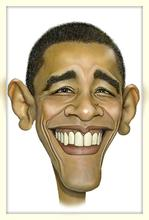
\includegraphics{obama.jpg}
            \caption{sb1}
        \end{minipage}%
        }
        \hspace{20pt}%
        \begin{minipage}{149pt}
            \centering
            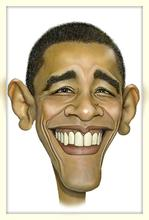
\includegraphics{obama.jpg}
            \caption{sb2}
        \end{minipage}
    \end{figure}

    %并排摆放,共享标题,各有子标题,使用subfig宏包的subfloat
    \begin{figure}[htbp]
        \centering
        \subfloat[xxoo]{
            \label{fig:subfig_a}
            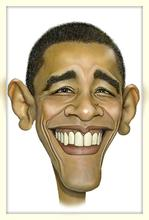
\includegraphics{obama.jpg}
        }
        \hspace{10pt}%
        \subfloat[ooxxxxxxxxxxxxxxxxxx]{
            \label{fig:subfig_b}
            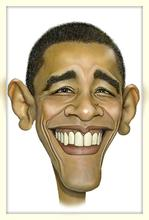
\includegraphics{obama.jpg}
        }
        \caption{sb xxoo}
        \label{fig:subfig}
    \end{figure}
        %当文档很长时,编译一遍也会很花时间。我们可以使用 syntonly 宏包,这样编译时就只检查语法,而不生成结果文件。
        %\syntaxonly不会用...

\end{document}
